\documentclass[12pt,a4paper]{report}

%%% User pakcages

\usepackage[font=scriptsize]{caption} %small caption text
\usepackage{wrapfig}
\usepackage{afterpage}
\usepackage{parskip} % Disable US-type paragraph
\usepackage{amsfonts} % Math 
\usepackage{palatino} % Vektor fonts
\usepackage{mathptmx}
\usepackage[T1]{fontenc} 
\usepackage[utf8]{inputenc} %%\usepackage[utf8x]{inputenc} 
\usepackage{float}
%\usepackage[danish]{babel} % Danish letters 
\usepackage{booktabs} % Nice tabels
\usepackage[pdftex]{graphicx} % Include graphics 
\usepackage{fancyhdr} % header & footer
\usepackage[hyphens]{url}
\usepackage[hidelinks, breaklinks]{hyperref} % Hyper link
\PassOptionsToPackage{hyphens}{url}\usepackage{hyperref}
\usepackage{titlesec}
\usepackage{xfrac}
\usepackage{listings} % Insert code
\usepackage[usenames,dvipsnames,svgnames,table]{xcolor}


\usepackage[backend=bibtex]{biblatex}
\bibliography{Kilder/kilder.bib}
\usepackage[left=2.5cm,right=2.5cm,top=2.5cm,bottom=2.5cm]{geometry} % Page margin
\usepackage{tabularx} % Table
\usepackage{marginnote}

\titleformat{\chapter}{\normalfont\huge\bfseries}{ \thechapter.}{20pt}{\huge}
\setcounter{section}{0}
\pagestyle{fancy}
\fancypagestyle{arabic}
{
    \fancyhf{}
    \setlength{\headheight}{15pt}
}

\renewcommand{\chaptermark}[1]{ \markboth{#1}{} }
\fancypagestyle{chp}{
  \fancyhf{}
  \rhead{\rightmark}%\colorbox{black}{\color{white}{\rightmark}}}
  \cfoot{\thepage}
}

\pagestyle{chp}

\title{Ground Handling}
\author{
    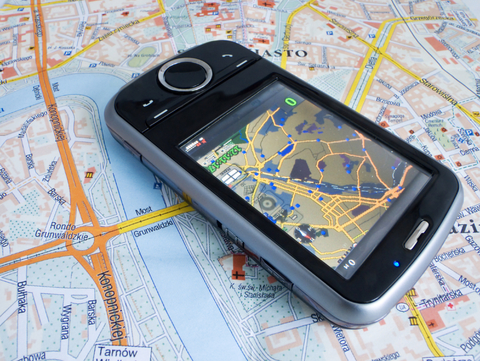
\includegraphics[width=14cm]{Grafik/index.jpg} \\
        Kasper Ø. Helsted, Jens H. Stærmose, Christoffer C. Christensen, Christian H. Nielsen\\
        Kasper F. Christensen, Anders L. Matthiassen \& Josias Laugesen\\
}
\date{21 - 05 - 2014}

\definecolor{codecomment}{HTML}{383838}

\lstset{language=C,
    basicstyle=\ttfamily\scriptsize,
    keywordstyle=\color{Blue}\ttfamily,
    otherkeywords={WIDTH},
    keywords=[2]{__shared__},
    keywordstyle=[2]\color{orange}\ttfamily,
    stringstyle=\color{red}\ttfamily,
    commentstyle=\color{codecomment}\ttfamily,
    breaklines=true,
    numbers=left,
}

\begin{document}
    \maketitle
    \afterpage{\null\newpage}
    \pagenumbering{gobble}
    \clearpage  
    %Titlepage 
    \thispagestyle{empty}
\begin{titlepage}
	\setlength{\textwidth}{15cm}
	\noindent
	\begin{nopagebreak}
		{\samepage 
			\begin{tabular}{lr}
				\parbox{0.5\textwidth}{\raisebox{11mm}
					{
\includegraphics[height=1.2cm]{Grafik/aauLogoDa}}
				} &
				\parbox{0.5\textwidth}{
					\small
					\begin{tabular}{l}
						{\sf\small \textbf{Institute of Computer Science}}\\
						{\sf\small Strandvejen 12-14, 9000 Aalborg} \\
						{\sf\small Telephone 96 35 97 31} \\
						{\sf\small Fax 98 13 63 93} \\
						{\sf\small http://tnb.aau.dk}
					\end{tabular}
				}
			\end{tabular}
			
			\noindent
			\begin{tabular}{cc}
				\parbox{7cm}{
					\begin{description}
			
						\item {\bf Title:} 
			
							\textbf{Ground Handling}\\
						\item {\bf Project Period:}\\
			  				Spring Semester 2014\\
			 				\hspace{4cm}
						\item {\bf Project Group:}\\
							SW2-A418\\
			  				\hspace{4cm}
						\item {\bf Participants:}\\
							Kasper Østergaard Helsted\\
                            Jens Hegner Stærmose\\
                            Christoffer Carlé Christensen\\
                            Christian Heider Nielsen\\
                            Kasper Fuglsang Christensen\\
                            Anders Lykke Matthiassen\\
                            Josias Laugesen\\
							\hspace{2cm}
						\item {\bf Supervisor:}\\
							Ramin Sadre\\

						\item {\bf Copies:}\\ 10\\
						\item {\bf Page Numbers:}\\ 65\\
						\item {\bf Appendix:}\\ None\\
						\item {\bf Number and Type of Annexes:}\\ 14 pages, code\\
						\item {\bf Date of Completion:}\\ 21-05-2014\\
					\end{description}
					\vfill
				} &
				\parbox{7cm}{
					\vspace{.15cm}
					\hfill 
					\begin{tabular}{l}
						{\bf Abstract:}\bigskip \\
						\fbox{
							\parbox{6.5cm}{\smallskip
								{\vfill{\small \section* {Synopsis}

								\smallskip}}
							}
						}
  					\end{tabular}
  				}
			\end{tabular}
		}\\
		\\
		\noindent{\footnotesize\emph{The content of this report is freely accessible, but publication (with referencing) may only happen under agreement with the authors.}}
	\end{nopagebreak}
\end{titlepage}

    \afterpage{\null\newpage}
    \pagenumbering{gobble}
    \clearpage  
    \pagenumbering{roman}
    \chapter*{Forord}


    %\renewcommand*\contentsname{Indholdsfortegnelse}
    \tableofcontents
    \thispagestyle{empty}
    \pagenumbering{arabic}
    \clearpage
    \setcounter{page}{1}
    \chapter{Indledning}

    \part{Problem Analysis}
    %\chapter{Problem Analysis}
		\chapter{Stakeholders}
\section{Organisations}
\subsection{Ground Handling Companies}
Ground handling companies are one of the primary stakeholders to consider, since they are the main target group for our project.

Ground handling companies provide an array of services for the airport and airlines. Among these are aircraft handling services, such as cabin cleaning, loading and unloading, luggage sorting and ULD control. Besides handling the aircraft, many also handle passenger services, such as check-in, lost and found and VIP services. Some ground handling companies even assist with weather briefing or flight operations.

For the ground handling companies to handle such a vast amount of services, they need a large number of employees carrying out a lot of different tasks. Managing all of these employees is therefore not an easy task, and can require multiple supervisors, making sure that each of the ground handlers is working efficiently and that they are not idle for prolonged periods of time. The job of managing this crew of ground handlers is usually done manually, where the supervisors distribute the workload among the ground handlers to the best of their ability, and assigning tasks to the ground handlers individually.
This method is far from ideal, as mistakes can easily happen when assigning tasks among large numbers of ground handlers, due to the supervisors being pressed on time, as to not delay the work of the ground handlers. These mistakes can potentially be catastrophic as they can lead problems ranging from delays, due to poor planning, to crucial errors in handling aircraft, due to assigning a ground handler to a task, which he does not have the required skills to perform.

To further clarify which specific problems arise when delegating tasks among the ground handlers, we will conduct an interview with a/some airport(s). These interviews and the results thereof will be described later.
		\section{Operational Personnel}
\subsection{Freight}
In this section the freight handled at airport will be analysed as the transportation of goods and passengers plays a major role in a everyday life of an airport. 

Luggage is loaded on the plane using tugs, which transport containers with luggage. The Boeing 747 has seats for 416 passengers\cite{freight_boing} and can carry roughly 6,500 kg of luggagem or 9,568 kg if the plane would be entirely booked and every passenger had a 23 kg checked luggage, as in the estimate the hand luggage is not being taken into account. To transport such a huge amount of luggage, tight planning and careful transport is necessary in order to bring the luggage onto the airplane in a timely fashion.

Novia and SAS Ground Handling are two ground handling companies that have the responsibility of loading luggage \cite{mistet_bagage}. If a passenger's luggage is, by mistake, sent with a wrong plane, the passenger can contact the airline company, and then they will talk with the ground handling company, that handled the luggage. In Aalborg Airport, luggage is equipped with a RFID chip that allows the Airport to track all luggage, and use that information in an advanced sorting machinery that has managed to almost eliminate loss of luggage.


Luggage isn't the only thing transported. Aside from passengers, cargo is a big part of aerial transportation and is an industry that has existed as long as passenger transportation. An increasingly growing part of the world trade is beginning to be transported by air and although a lot of people have the notion that most cargo is transported in separate airplanes, actually more than 60\% of all cargo is transported in passenger flights in the unused space besides passenger luggage. %Kilde mangler stadig Carle?


Besides the passenger flights an increasing proportion of cargo is transported by integrated (where the airlines or other companies have their own equipment and airplanes) or express (Where it is handled as additional luggage) 
carriers by a so-called door-to-door service, where the company transport the goods all the way. Since the companies that transport the cargo is in charge of all the transportation, both in air and on ground, the tracking of cargo is a lot easier and the direct involvement of the costumer is kept to a minimum. Their services mostly take shipments less than 100 kg. This service help the larger companies transport cargo a lot easier. For instance FedEx delivers 3.2 million packages per day in more than 220 countries through 50,000 drop-off locations, using 671 aircraft, 41,000 vans and 138,000 employees (2005). %Kilde mangler

Many integrators, companies using integrated carriers, construct and operate their own terminal where their goods arrive and is checked, packed, documented, transported to the apron and so on by their own system. 
Their traffic is normally very peaky and the dwell time is normally shorter. Their goods normally consists of packages smaller than 30 kg and courier mail. At these terminals the standards are normally:
\begin{itemize}
\item Consignments available for collection, examination or transhipment(ready for collection) three hours after arrival
\item Cleared consignments available within 15 minutes of consignee arriving at import collection point
\item Customers to not wait more than 30 minutes after arrival for collection at truck dock
\item Cargo reception to be complete within 30 minutes of arrival at truck dock
\end{itemize}

("It is quite common for integrators to use space on combination carriers and vice-versa. There are also airlines that specialise in heavy lift, using small fleets of unique aircraft like the AN 124 or the Mil 10 helicopter.") %WTF?

When cargo arrives at the airport it normally arrives at a terminal, it is normally transported via electrical tugs from the trucks into the terminal in carts carrying bulk cargo, pallets or containers. The cargo is now taken through a sorting process that deposits the goods directly at the stuffing platforms or they are again taken by conveyor (packages up to a maximum of 30 kg are put into trays on the conveyers) or fork lift to the platform.
Unless the container for a destination is full, the cargo is rearranged at these platforms by destination in new containers called ULDs, which stands for Unit Load Device and is normally a pallet or container, specific for the aircraft type it needs to be transported on.


This also applies to cargo arrived from air from another air plane where the cargo is in transit in the current airport. The only difference being that this cargo arrives from the air side, not the land side.
This process of rearranging is entirely manual, no matter how mechanized the terminal is (will be described shortly) and is preferably done on height-adjustable platforms that can indicate the weight and sometimes the stability of the ULD. This information is very important when you load the aircraft to ensure a stable aircraft in balance.


There are five different tasks performed in the terminal:
\begin{itemize}
\item Conversion between modes of transport
\item Sorting, including breaking down loads from originators and consolidating for destinations
\item Storage, and facilitating government inspection
\item Movement of goods from landside to airside and vice-versa, or from aircraft to aircraft
\item Documentation: submission, completion, transmission
\end{itemize}

Getting these five tasks just right and performed smoothly and effectively can reduce the mishandling rate from 1 : 20 to 1 : 26,000.

Normally the terminals use the storage area to store cargo, which is awaiting clearance, but it is also used for cargo before it is rearranged or outbound cargo awaiting consolidation, stuffing or simply waiting for its departure time and transhipments. This pickup can be a matter of an hour or two, but can in some countries be several weeks, if they have no restrictions since it is essentially free storage for the companies. This, in developed worlds, is normally not the case, where the time is normally 20 hours for export, 40 hours for import and 32 hours for transhipment. %er dette afsnit på nogen måde relevant?? samme med de følgende 3

In total, an order takes about 6 days from sender to receiver, where the cargo normally spends 90\% of its time on the ground where 12\% is transport time and the rest is storage, where the cargo is waiting on documentation due to lack of resources or information, inaccurate delivery instructions or problems with customs clearance. This stands very much in contrast to the inside of the integrators' terminal where cargo normally arrives just before it is time to be shipped by plane and has already been cleared and sorted.%mange procenter uden kilder

All cargo can at all times be forced to be inspected by government agencies for contraband, drugs, illegal immigration, weapons and so on.

In different countries they have different standards for labour and the level of automation in the terminal is therefore different in each country. Generally there are three different levels of mechanization.
\begin{itemize}
\item Manual: Manpower plus fork lift trucks
\item Semi-mechanised: Roller beds or conveyors
\item Fully mechanised: Elevating Transfer Vehicles (ETV), Automatic Storage and Retrieval Systems, Transfer vehicles
\end{itemize}

("A semi-mechanised system possibly have a conveyor systems and powered flat roller conveyors where the rollers are chain-driven from the previous one. They will also have reorienting and transfer dock beds: some have wheels that right angles rise up between the rollers, or powered ball decks, or heliroll rotation tables where the different quadrants are powered with a joystick.") %SOMEBODY??

The benefits of a manual and mostly labour controlled system is that it is flexible in peak-hours and can easily adjust but the  disadvantages is that is is more expensive over time.
On the other hand, a fully mechanised system functions best when a lot of cargo flows through the terminal and all of this is containerised and the machines can be serviced very fast. Of cause the whole system can still break down if an ETV (Elevating Transfer Vehicle; the vehicles that organise multilevel storageup to seven meters) breaks down.  Therefore for instance British Airways, also use lifts and lowered roller conveyors at it's multi-level World Cargo Centre at Heathrow, in case of a breakdown.

Normally cargo is transported to the flights at the so-called aprons which is the area where the flight is serviced by the ground handlers, usually via trucks, though some airports also use rail.

This cargo and luggage is normally transported in ULDs via roller-bed dollys (Flat carts acting as wheels for the ULDs) to the aircraft and then lifted into the aircraft either from the side or the front via high-loader vehicles (A truck specialised to raise and move the ULDs inside the aircraft).
The ULD can now be organised inside the aircraft on roller beds (a small track-like system consisting of small cylindrical "wheels" where the ULD can be pushed). The cargo needs to be loaded in the right order to achieve balance. The bulk cargo (cargo that is not containerized or on pallets), which have been transported to the flight in carts, can now be loaded into the flight via self powered conveyer belts. Therefore is it very important for the airport to know if the cargo will arrive in bulks, on pallets or on ULDs and if it needs transportation from the terminal to the apron, or the company will transport it on trucks, granting access to the aprons.
%Et billed af de ULD's vil være godt?

%Nedenstående: Hvad er "this equipment"?
This equipment is very expensive, especially the high-loaders, which needs specialised drivers; as a result, the companies often share this equipment.

There is a lot of movement between the cargo and passenger aprons and they should therefore be placed close to each other.%relevant?

Research:
\begin{itemize}
\item How much cargo is normally transported?
\item How expensive is it to have you airplane in the airport in fees? ("Time in flight and in transit is most important, a saving of one hour perhaps being worth \$1000 in airport fees. (2005)")
\end{itemize}


Knowledge (2005):
\begin{itemize}
\item The trends also tend to reduce the ratio of value to weight, but the aircraft loads are still generally more limited by volumetric capacity than by weight limits.
\end{itemize}

In conclusion; the amount of freight, consisting of cargo, mail and passengers, are present everyday in multiple tons. The personal and ULD's are working precisely  in order to make sure the freight is transported to the right locations and flights. The cargo can not wait for too long at the storing areas as there is a certain time limit at  most airfields. A fully mechanised system will be able to service containers and machines in a very fast manner, as a lot of these flows through the terminals.

		\subsection{Air plane Mechanic}
To be able to make a thorough analysis of the personal involved in the handling and maintenance of the flights, it's necessary to take a look at the relevant workers. Mechanics are the workers handling maintenance, and in this chapter their job and the potential for optimization of this, will be evaluated.

The air plane mechanic has a very important job in the airport, their job is to repair the air planes. It's therefore important that these working crews can access the air plane that needs repairing quick and easy, and know where they needs to go, so the air plane can get flying again as quickly as possible. It is also important that they do their job as good as possible, as every part needs to be maintained correctly.

In Scandinavia and the Baltic countries, the leading air plain mechanic company regarding technical air plane maintenance is SAS Tech\cite{sas_tech_mechanic}.

If it would be possible for air plane mechanics to know exactly where to go by viewing it on a smartphone, PDA or other portable device, the mechanics would be able to be more productive, as they would know instantly where they where needed for their next task. 

Boeing has released an application to help the mechanics get important things like air plane manuals, and serial numbers for specific parts. If they would be able to do this with every air plane, or every air plane at Aalborg Airport, it would help the mechanics tremendously as they would be able to identify the parts they needed much quicker, and therefore the maintenance of an air plane would be quicker. By using an application you would also be able to find earlier maintenance records, meaning that if another mechanic may have made a mistake, you would be able to identify it much quicker\cite{cnet_boeing_app}.

A downside to making an application like boing, could be the obvious problem of grease. If the Mechanics are supposed to use a tablet, PDA or smartphones, wouldn't they need to use a lot of time to clean their hands in between using the device, and would this really make the repairing of the aircraft faster?

Other suggestions for application that could help mechanics do their job faster an better include:
\begin{itemize}
\item An application that gives suggestions how to fix things by describing the problem (Ex. Weird Noise in Cabin)
\item An application that would help them calculate different things, like what to setting to set the torque screwdriver to. \ldots
\end{itemize}

After this has been checked it can be concluded that the only area that can be easily implemented in a software solution, would be the manuals and serial numbers part.

		\section{Cabin Crew}
In this section the focus will be put on which tasks and responsibilities the cabin crew takes on. 

Ahead of each flight, the entire flight crew are required to show up to a briefing about the flight.

At the briefing, the crew undergoes the safety protocols, emergency checklists, the targeted location, and how much safety equipment are onboard the flight. The flight personal is in charge of boarding V.I.P. passengers, families with small kids, and passengers with special needs.

Once a plane has taken off, the crew serve drinks and food to the passengers. While they serve food and drinks, it is also their responsibility to periodically conduct cabin checks and listen for any unusual noise. Additional task of periodic checks and restock of lavatories, here the crew investigates the mandatory ashtray and if smoke detectors have been tampered with. In addition, the cockpit needs to be checked regularly ensure the pilot's health and safety. Before each landing, the crew gather food trays and rubbish to disposed before the final landing procedure is initiated, fastening all loose items and a final cabin check is concluded.

To get the education, it is a requirement to have been an employee of an airline company. It is the company’s responsibility to educate the employee. 

Some of the important aspects about the cabin crew, are that they

		\section{Supervisors}
The supervisors to the ground handling teams are very important stakeholders to consider, when developing programs which apply to ground handlers.

The supervisors have to direct the ground handlers effectively, and monitor their performance level. Therefore it is the supervisors, who bear the main responsibility if the program is ineffective or decreasing in performance. If the program should be any of the aforementioned, the supervisors probably have the biggest say in deciding whether to terminate the use of the program or not.

For the program to be most relevant for the supervisors, it should be designed with features that ease or simplify the workload of the supervisors. That could be features like motivating the workers, dynamically allocating tasks among the workers and/or making performance evaluation reports easily available to the supervisor.
		\section{Cleaning}
Cleaning is a large part of the routine the plane is undergoing when it arrives to the airport.

%billede -> timetable
%text: Timetable, shown without tavel time
Which makes the cleaning companies a very intersting part to take a look at.

The time it take to clean the cabin, is roughly half of the time the plane is standing still, according to the timetable.

Depending on the time it takes to tavel to the aircraft, it can take longer than shown on the timetable.



%need moare infomation from AAL airport



		\subsection{Catering} 
Catering crews are yet another part of the ground handling crews. It is therefore interesting for this project to look into how their workday is structured.

When passengers are on long flights, there will be served air meals for them, most of which consist of different kinds of meat, vegetables and drinks. The pilots are served with the same dishes, although this varies in between the different airlines\cite{cate_pilotfood1}\cite{cate_pilotfood2}. SAS offer breakfast when flying domestic flights, but only from 6 to 9 AM\cite{cate_SASIndri}. When flying in between Scandinavian and other European countries, there will always be served coffee or tea, but in order to get breakfast served the passenger has to be a member of premium service\cite{cate_SASscanda}.

All these air meals and drinks are prepared and made by the catering services, that are a part of the ground handling organization. The catering companies are chosen by the different airlines individually. SAS for example, have used Gate Gourmet\cite{cate_SASGourmet} as their catering service for a number of years. The catering services are very difficult in the sense of how complex the logistic aspect is, as the President of KLM Catering said "Flight catering is 70 
percent logistics and 30 percent cooking”\cite{cate_BookSection}. For this reason the catering services want their operations to go as smoothly as possible. The airline companies are also very interested in getting capable catering services, as they can then use the food as a marketing technique\cite{cate_BookSection}. 

Since logistics are so essential to the catering crews, a way to optimize their workday would be very beneficial for the catering companies, both by making the teams more efficient and by making the logistics aspect simpler.
		\subsection{Passengers}
When talking about air traffic it is of cause also very important to find out what the passengers themselves want, therefore this part of the report will look at what passengers think is the most important things for them in a flight.
In a survey made by eNT - Global Travel Industry News, they asked more than 3.200 people what they thought is the most important thing in their flight.
\begin{itemize}
\item 25\% - thought limited legroom was one of their biggest gripes about air travel
\item 30\% - lobbied for more legroom
\item 38\% - requested roomier seats
\item 25\% - consider airline fees to be their biggest complaint about air travel
\item 56\% - thought checked baggage fees were the most annoying current airline fee
\item 56\% - expect the overall cost of airline fees to rise in 2010
\item 74\% - think passengers of size should be required to purchase tickets for two seats on their flights
\item 21\% - think that airlines will add passenger of size fees in 2010
\item 30\% - they would be more likely to book a flight on an aircraft with in-flight Wi-Fi than one without
\item 61\% - they would not be willing to pay for in-flight Wi-Fi access
\item 27\% - they would be willing to pay \$5 or less for the service
\item If the person sitting next to them on their flight were accessing inappropriate content on their computer using in-flight Wi-Fi:
\begin{itemize}
\item 45\% - would do nothing
\item 27\% - would alert a flight attendant
\item 22\% - would ask their seatmate to close the inappropriate content
\item 6\% - would file a complaint with the airline
\end{itemize}
\item With the rise of checked baggage fees:
\begin{itemize}
\item 58\% - said they always or often carry on their bag to avoid extra charges, possibly adding to cramped overhead bins
\item 62\% - said they would put their carry-on bag above someone else's row if their own overhead space were already filled
\item 57\% - said that each seat on a plane should have assigned space in the overhead compartment, even if it meant carry-on bags had to be smaller
\end{itemize}
\item 79\% - said they are comfortable with U.S. airports using full body scanners that can see through clothes
\item 52\% - prefer the aisle seats
\item 44\% - favor the window seats
\item 33\% - request seats in the exit row on their flights
\item 13\% - ask for bulkhead seats
\item 39\% - cite long security lines as the most annoying part of being at an airport
\item 19\% - think that airports have high prices for food
\item 14\% - think that there is not enough seating in the boarding area
\item 95\% - think there should be a price limit on bottled water post-security at the airport, since security checkpoints require passengers to leave larger bottles behind
\end{itemize}

\subsection{Control during the journey [CHANGE!]}
Passengers want control over and knowledge about their journey on the run. A survey made by SITA (have no clue what it is a abbreviation for) in 2012 [http://www.sita.aero/content/airline-passengers-want-more-control] shows that 90\% of the 2,526 passengers included in the survey thinks that flight status updates on their mobile phones and self-boarding is their absolute top technologies when it comes to air travel. Furthermore an increasing rate of the world's population is getting smart phones and therefore also the rate of passengers. The number of passengers who has a smart phone went from 54\% in 2011 to 70\% in 2012 and is expected to reach 90\% in 2015. Therefore it it clear that the market for smart phone applications for the passengers witch can keep them informed about their flights, delays, boarding hours ect. and which they can also use to check-in and get their boarding passes from is something most airports and/or airlines should try to make. Already 21\% og passengers are now using mobile boarding pass.
Another survey made by IATA in 2012 shows that only a very small procentage uses the Airline application for smartphones to book their flight whereas 52\% books online via the airline website, see figure \ref{channes used to book}.

\begin{figure}
\centering
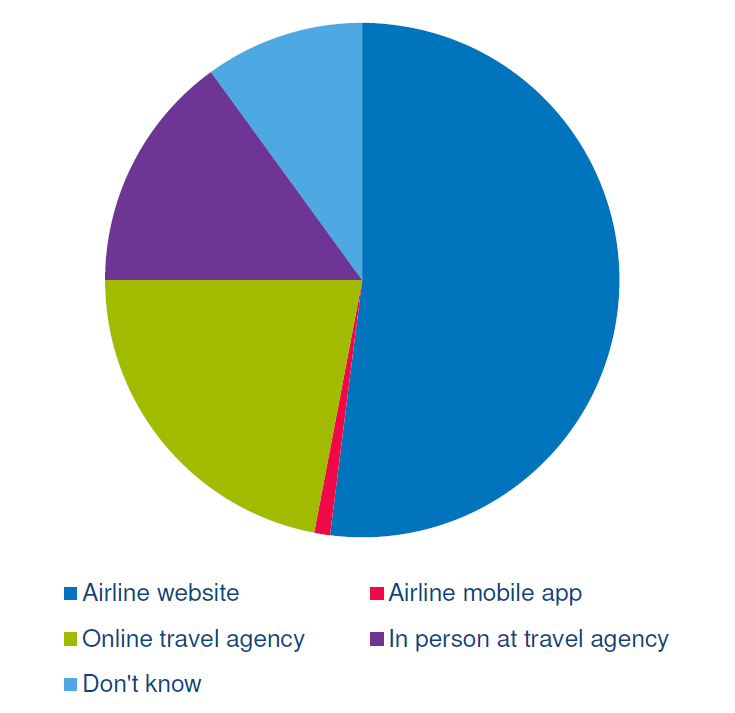
\includegraphics{Grafik/channes_used_to_book}
\caption{Breakdown of channels used to book flights.}
\label{channes used to book}
\end{figure}

%Kilder:
%http://www.iata.org/publications/Documents/2012-iata-global-passenger-survey-highlights.pdf
%http://business.time.com/2012/09/20/airline-introduces-perk-passengers-actually-want-and-its-free/
%http://consumertravelalliance.org/2011/02/06/what-do-airline-passengers-really-want-%E2%80%94-besides-a-good-fare/
%http://www.eturbonews.com/14902/survey-what-passengers-want-airlines
%http://elliott.org/blog/what-do-airline-passengers-really-want-besides-a-good-fare/
%http://blog.apex.aero/inflight-services-2/ten-premium-passengers-airlines/



		
		\subsection{Airports}

In the following section, airports, mainly Aalborg Airport, will be described. THe section will go into the prices and services of Aalborg Airport, describing prices on things like fuel. In the section it will also be described how the emergency protocols of big airorts are, and how these are supposed to be handles. Furthermore the section look at the types and amount of airplanes travveling through Aalborg Airport, and at last it will be described how the teams at Aalborg airport is managed, and how this could be bettered.

\subsubsection{Prices and Services}
When designing products aimed at airports, it is interesting to find out what services and what prices the airports usually deal with. In this section we will look at different prices and services in airports.


Fueling is an important part of ground handling, since refueling it is a task that must be performed every time a planes arrives. Aalborg Airport has an agreement with the Shell corporation, to get their fuel supply from them. The air planes are fueled with a fuel type called 100LL \cite{iaopa_fuelprices}, and is a very common aircraft fuel, it is priced at DKK 19.85 pr. litre, which means that if you would have to fill up a Boeing 737-800, which can contain 26,020 litres\cite{737_specs}, it would cost DKK 516,497 plus the start up fee.

As described above it is clear that there is a lot of money going around in an airport, even when only one air plane is taken into account. The air planes need to get filled up before every lift off, since a Boeing 737-800 uses 3,200 litres of fuel pr. hour when it is in the sky. This means that if you were to fly from Aalborg to Copenhagen it would cost, just in terms of fuel, DKK 47,640, as it takes 45 minutes to fly from Aalborg to Copenhagen.


According to Aerohandlers' pricelist (%source http://www.aerohandlers.com/download/aerohandlers_pricelist.pdf)
, airlines pay upwards of USD 3000 for a single airline to have ground handling performed upon. This indicates that the cost of performing ground handling, for the ground handling companies, is also very high. If you were able to optimize ground handling procedures, then costs for the ground handling companies could be reduced, leading to lower prices for the airlines and ultimately lower prices for the passengers. Therefore, optimizing the work flow on ground handling procedures is a very relevant aspect of designing solutions for aiports.
    \section{In case of an emergency}

Occasionally an unexpected emergencies at airport incurs, the airport needs to respond to. A standard service manual for handling potential emergencies exists, for the relevance of this project it is interesting to know how to handle and maintain emergency landings. Which runway to shut down and prepare for the emergency, how to handle incoming and outgoing traffic and other airport services.
The manual suggest following plan for an aircraft accident on the airport:



In general alot of different (organisations / agencies) is involved in these emergencies, each with their own responsibilities. The airport traffic services includes following:

\begin{quotation}
Chapter 4
RESPONSIBILITY AND ROLE OF EACH AGENCY FOR EACH TYPE OF EMERGENCY

4.1 AIRCRAFT ACCIDENT ON THE AIRPORT
4.1.1 General
The airport emergency plan shall be implemented immediately upon an aircraft accident occurring on the airport. For this
type of emergency, responding agencies are expected to take action as described in 4.1.2 to 4.1.10 below.
4.1.2 Action by air traffic services
4.1.2.1 Initiate emergency response by using the crash alarm communication system (See Figure 8-1).
4.1.2.2 Notify the rescue and fire fighting service and provide information on the location of the accident, grid map
reference and all other essential details, including time of the accident and type of aircraft. Subsequent notification may
expand this information by providing details on the number of occupants, fuel on board, aircraft operator, and any
dangerous goods on board, including quantity and location, if known.
4.1.2.3 Close the affected runway and minimize vehicle traffic on that runway to prevent disturbance of accident
investigation evidence (See 4.1.5 2) f)).
4.1.2.4 If required, initiate communications to the police and security services, airport authority, and medical
services in accordance with the procedure in the airport emergency plan. Provide the contacts with grid map reference,
rendezvous point and/or staging area and airport entrance to be used.
4.1.2.5 Issue the following Notice to Airmen (NOTAM) immediately:
“Airport rescue and fire fighting service protection unavailable until (time) or until further notice. All equipment committed
to aircraft accident.”
4.1.2.6 Verify by written checklist that the actions above were completed, indicating notification time(s) and name
of person completing action.



4.3 FULL EMERGENCY
4.3.1 General
The agencies involved in the airport emergency plan shall be alerted to “full emergency” status when it is known that an
aircraft approaching the airport is, or is suspected to be, in such trouble that there is a possibility of an accident.
4.3.2 Action by air traffic services
4.3.2.1 Notify the airport rescue and fire fighting service to stand by at the predetermined ready positions
applicable to the planned runway and provide as many of the following details as possible:
a) type of aircraft;
b) fuel on board;
c) number of occupants, including special occupants — handicapped, immobilized, blind, deaf;
d) nature of trouble;
e) planned runway;
f) estimated time of landing;
g) aircraft operator, if appropriate; and
h) any dangerous goods on board, including quantity and location, if known.
4.3.2.2 Initiate notification of the mutual aid fire department(s) and other appropriate organizations in accordance
with the procedure prescribed in the airport emergency plan, providing, if necessary, the rendezvous point and airport
entrance to be used.



4.4 LOCAL STANDBY
4.4.1 General
The agencies involved in the airport emergency plan shall be alerted to “local standby” status when an aircraft
approaching the airport is known or is suspected to have developed some defect but the trouble is not such as would
normally involve any serious difficulty in effecting a safe landing.
4.4.2 Action by air traffic services
Notify the airport rescue and fire fighting service to stand by as requested by the pilot, or stand by as local airport
agreements require at the predetermined ready positions applicable to the runway to be used. Provide as many of the
following details as possible:
a) type of aircraft;
b) fuel on board;
c) number of occupants, including special occupants — handicapped, immobilized, blind, deaf;
d) nature of trouble;
e) planned runway;
f) estimated time of landing;
g) aircraft operator, if appropriate; and
h) any dangerous goods on board, including quantity and location, if known.
\end{quotation}


In conclusion a runaway is assigned to the "full emergency" and the "local standby" statuses, and when an accident incurs the affected area is closed and traffic through area is minimized. Also a signal of NOTAM are issued to notice that airport rescue and fire fighting services are all currently occupied.



-source
Airport Services Manual, Part 7 by International Civil Aviation Organization (ICAO)
Second Edition - 1991


		\section{Airtraffic from Aalborg Airport}

By 2013 there where more then 6.000 official airline flights from Aalborg airport, of them, the most common types of aircrafts are shown in the table below:

\begin{center}
    \begin{tabular}{ | l | c | }
        \hline
        Aircraft & Flights\\ \hline
        BOEING 737-800 & 2919\\ \hline
        AIRBUS A-320 & 2544\\ \hline
        FAIRCHILD DORNIER 328 & 1080\\ \hline
        EMBRAER ERJ 190-100 & 732\\ \hline
        AIRBUS A-321 & 725\\ \hline
        FOKKER 70 & 723\\ \hline
        SAAB 2000 & 370\\ \hline
    \end{tabular}
\end{center}


Aalborg Airport, also have a private airtaxi service called North Flying, which can fly private passengers [http://www.aal.dk/b2b/north-flying/\#.UveuHvldVYU].

2.500 cargo flights are made daily [http://www.aal.dk/b2b/cargo-fragt/\#.UveuFfldVYU].



		
		\section{How to avoid bad planning}
In this section bad planning will be described, as a number of significant consequences follow if different tasks and jobs are poorly planned. Tools to overcome bad planning will also be described.

%Der mangler en kilde til "consequences resulting in outcomes such as, plane delays, lost income, stress, etc."
Bad planning can have different consequences resulting in outcomes such as plane delays, lost income, stress and so forth. It is therefore important that the planning is as efficient as possible, to ensure that the ground handling companies can perform all their tasks in the desired time frame.

To avoid bad planning, it is important to utilize different tools. These tools are described in \textbf{"INSERT REFERENCE"}. Avoiding bad planning does not necessarily suggest that one would have to make adjustments to the current way of handling different operations, however it could be necessary that one would need to come up with new ideas on how to avoid bad planning.

%Der mangler kilde til "...to give them a PDA, smarthone or tablet, and write out the job on the device"
%Der mangler en kilde til "This would make sure that they have understood the job properly."
Tom Mochal who is president of TenStep \cite{AvoidP_TenStep2} says that one of the major things that can make projects fail, or take longer time than needed, is the way that not all job are defined well enough. One way it could be made more clear to the people working on the project or job, is to give them a PDA, smartphone or tablet, and write out the job on the device. This would make sure that they have understood the job properly.


Another method that could be used, would be to give the employees the first part of a day to make sure that they had properly understood all the tasks that they are to do that day.

In conclusion; bad planning should be avoided in order to minimize plane delays, lost income and stress. An electronic device could help the employees to get a better understanding of what they have to do at the job. 
		\section{Consequences of Bad Planning}
Bad planning in a business aspect has an array of consequences. The direct effects of bad planning, in the context of ground handling companies, could be inefficient schedules for the ground handlers, not being properly prepared for emergencies and/or difficulties attaining performance reports on the ground handlers.

These direct consequences do not stand for themselves. Each of these cases give rise to an entirely new sprout of indirect consequences.
Looking at the case of inefficient schedules for the ground handlers, we need to define what it means for a schedule to be inefficient. Here there are three different cases
\begin{itemize}
	\item The duties on the schedules could be too close to each other
\end{itemize}
This means that the ground handler does not have the time to finish the first task without delaying the next. Consequences for this case includes amongst others, stress for the ground handler, delays in the overall handling schedule for the day and less productive days than anticipated by the supervisors.
\begin{itemize}
	\item The time it takes for a ground handler to move from task A to task B could be underestimated
\end{itemize}
This case has some of the same consequences as the first one. If the ground handlers suddenly has less time to do what he needs to than he had anticipated, he will become stressed and the second task would be delayed amongst.
\begin{itemize}
	\item 
\end{itemize}
		\section{Stress}
When dealing with work related stress the biggest causes are normally organizational factors, and the solution is normally to gain control through prevention and management.

When trying to understand stress it is important to understand that a situation can only be potential stressful depending on the person experiencing it. That means that a situation can evoke stress for one person, but the same situation can have no effect for another, depending on their way of handling understanding and viewing the situation. Aside from the person normally timing frequency, intensity and duration, are factors that determinate how big of an impact a potential stressful situation can have on the person.

"Stress can also have a considerable organisational and economic impact."

HSE's  longitudinal studies of occupational stress shows that 

"HSE's  logitudinal studies of occupational stress using changes in naturally occurring work situations have provided evidence that over quite short periods of time the nature of the work situation to which the person is exposed has significant effects on mental health quite apart from contributions from personality and pre-existing psychological health."

When dealing with work related stress an organization first need to manage and treat people on an individual level meaning that they first need to treat the people that are already stressed\cite{control_stress_work}.

After treating the individuals the organization need to approach its employees with interventions that restructuring the work flow. Organization of work tasks and inform their employees about the situation and how to deal with these changes. This approach is also very preventive for future problems, and can lead to, new work tasks and flow if it is done correctly, the potential stressful situations can be completely removed thereby removing the problem.

At this time the importance of training the individuals in managing potential stressful situation themselves, must be noted and it is largely accepted that this is the key for a healthy workforce. Also because interventions can be very costly in short term and may not even work or even make the problem worse, if for instance the new work plan is even more stressful.

Individual stress management focus on biofeedback, muscle relaxation and cognitive restructuring of appraisal and coping responses. This is a good approach because:

\begin{itemize}
\item They can quickly be evaluated and established without needing to change any organizational structure or work flow.
\item "They can encompass the need to take into account perceptions and reactions and are thus particularly appropriate for individual needs."
\item "They may be helpful in combating non-work as well as work-based stress problems (which may interact synergistically)."
\item "They can be incorporated into existing employee assistancehealth education packages."
\end{itemize}

One of the problems when dealing with stress as an individual, is to understand the complex situation with all the work and non-work related factors the contribute to ones mental health and their feelings of uneasiness or distress. Most people will need help from specialist to unravel this.

When combating stress in work-related situations on an individual, the organization can either help the person cope and handle poorly designed work methods or tasks or "the person to regain a degree of normal functioning so that return to productive working can be achieved."

"Moreover the impact of stress inoculation training may decrease over time leading to the need for repeated refresher training."

"The suggestion from some quarters is that stress management training should only be used to supplement organisational changd job redesign programmes inorder to deal with stressors which cannot be designed out of the job very easily, for example, seasonal workloads. Thus management at the secondary level should be used to supplement attempts to assess and restructure sources of stress in the work environment- organisational, ergonomic and psychosocial."
		\section{Motivation}
Activities that are not interesting (i.e., that are not intrinsically motivating) require extrinsic motivation, so their initial enactment depends upon the perception of a contingency between the behaviour and a desired consequence such as implicit approval or tangible rewards.

When externally regulated, people act with the intention of obtaining a desired consequence or avoiding an undesired one, and are thereby energized into action only when the action is instrumental to those ends (e.g., I work when the boss is watching).

Motivation involves having no intentions for the behaviour and not knowing why one is doing it. Research using this assessment strategy has confirmed that, in domains such as education (Williams \& Deci, 1996),

We argued earlier that the needs for competence and autonomy underlie intrinsic motivation that people need to feel competent and autonomous to maintain their intrinsic motivation. Experiments were reviewed that provided support for that proposition.

The need for relatedness is also crucial for internalization (e.g., Baumeister \& Leary, 1995). More specifically, SDT postulates that when people experience satisfaction of the needs for relatedness and competence with respect to a behaviour. They will tend to internalize its value and regulation, but the degree of satisfaction and the need for autonomy is what distinguishes whether it is identification or integration, rather than just interjection, will occur.

Using this definition, the needs for competence, autonomy, and relatedness are considered important for all individuals,

The work climates that promote satisfaction of the three basic psychological needs will enhance employees intrinsic motivation. This will promote full internalization of extrinsic motivation and will in turn yield the important work outcomes of persistence and maintained behaviour.
Particularly on tasks requiring creativity, cognitive flexibility, and conceptual understanding,job satisfaction,) positive work-related attitudes, organizational citizenship behaviours and psychological adjustment and well-being.


Hackman and Oldham (1980) argued that the most effective means of motivating individuals is through the optimal design of jobs.

The authors proposed that the means for increasing internal work motivation is to design jobs so they will (1) provide variety, involve completion of a whole, and have a positive impact on the lives of others; (2) afford considerable freedom and discretion to the employee (what action theorists refer to as decision latitude); and (3) provide meaningful performance feedback.

constructive feedback as one way to influence autonomous motivation, but it also suggests that the interpersonal style of supervisors and managers is important.

Pertinent to this is the finding that jobs with high motivating potential scores were associated with enhanced psychological states and better outcomes only for workers who perceived that pay and promotion were not contingent on performance (Johns, Xie, & Fang, 1992).

studies have found that managers autonomy support led to greater satisfaction of the needs for competence, relatedness, and autonomy and, in turn, to more job satisfaction, higher performance evaluations, greater persistence, greater acceptance of organizational change, and better psychological adjustment (Baard et al., 2004; Deci et al., 2001; Gagne´ et al., 2000; Ilardi, Leone, Kasser, \& Ryan, 1993; Kasser, Davey, & Ryan, 1992).

Bono and Judge (2003) showed that followers of transformational or visionary leaders were more likely to adopt autonomous goals than controlled goals in the workplace. These followers were also more satisfied with their jobs and more affectively committed to the organization.

Taken together, studies in organizations have provided support for the propositions that autonomy-
supportive (rather than controlling) work environments and managerial methods promote basic need satisfaction, intrinsic motivation, and full internalization of extrinsic motivation, and that these in turn lead to persistence, effective performance, job satisfaction, positive work attitudes, organizational commitment, and psychological well-being.


Together, the studies suggest that autonomous motivation, consisting of a mix of intrinsic motivation and internalized extrinsic motivation, is superior in situations that include both complex tasks that are interesting and less complex tasks that require discipline. When a job involves only mundane tasks, however, there appears to be no performance advantage to autonomous motivation. Still, even in those situations, autonomous motivation will be associated with greater job satisfaction and well-being, as was found by Ilardi et al. (1993) in a study of employees with monotonous jobs in a shoe factory and by Shirom and colleagues (1999) in a study of blue-collar workers with mundane jobs. This implies that, overall, autonomous motivation is preferable in organizations because even with dull, boring jobs there is an advantage to autonomous motivation in terms of job satisfaction and well-being, which are likely to yield better attendance and lower turnover (Breaugh, 1985; Karasek & Theorell, 1990; Matteson \& Ivancevich, 1987; Sherman, 1989).

research suggests that intrinsic motivation (based in interest) and autonomous extrinsic motivation (based in importance) are both related to performance, satisfaction, trust, and well-being in the workplace.
		
		\chapter{Problem Statement}

Ground handling companies often hire low-paid workers, who work in an environment where they are exposed to congestion, stress, noise, jet-blast, extreme weather conditions and sometimes low visibility. Stress is a very factor in the work in an airport, especially to the ground handlers, since airline companies only make money, while the flights are airborne, therefore the ground handlers are very pressed on time, to reduce the time the flight spends on the ground. In many places it is also the ground handlers, who are responsible for delays; in case of a delay, they might even be deducted in salary.

When a worker is stressed he is more likely to make mistakes, which could lead to serious accidents. These accidents can first and foremost become dangerous for the workers because they can be hurt as a result of an accident. A survey made by ACI[citation needed] in 2004 showed that out of 15,119,020 aircraft movements 3,233 had accidents, concluding that 0.214\% of all turnovers had accidents.

Accidents do not only lead to dangerous situations for the workers, but they can also get very expensive for the companies; first of all because of the cost of the repair, but also because the aeroplane will then have to spend more time on the ground.
\section{Problem Formulation}
\begin{center}
\textit{Human errors and accidents during a turnaround is a result of stressed and unmotivated employees, causing delays, damage to equipment, loss of airtime and other unwanted annoyances for airlines and ground handling providers. Is it possible to formulate a software solution to resolve these issues by dynamically adapting to non-scheduled situations?}
\end{center}

		
		\chapter{TEMP}
    \subsection{Stakeholders} 
\label{Stakeholders}

Personal
\begin{itemize}
\item Security
\item Flight controllers
\item Emergency crew
\item Clean up crew http://alturl.com/3onjh
\item Catering staff
\item Mechanics
\item Flight Crew
\item Baggage handlers
\item Boarding Personal
\end{itemize}

The Airport
\begin{itemize}
\item Administrators
\end{itemize}

The Airline companies
\begin{itemize}
\item SAS, Lufthansa, Norwegian, etc...
\end{itemize}

Passengers
\begin{itemize}
\item Check-in
\item Delays
\end{itemize}
	
\section{Organization}
\label{Organization}
Supply chain(Fuel, Water, Food )	
Infrastructure(Taxiing, Gates)
	
\section{Technology}
\label{Technology}
Computers
Smartphones
GPS
Internet(Servers)
Databaes(Arrivals, 

\section{Existing Solutions}
\label{Existing Solutions}
(FILL IN LATER!)

\section{Solutions}
\label{Solutons}
Make an information system to achieve:
\begin{itemize}
\item Optimized infrastructure(Taxiing, Passengers, Fuel)
\item Prices(Total Price for ground handling services)
\item Servers bases solution, accessible on various platforms/interfaces
\item Passenger handling(Baggage Boarding, Food, Water)
\end{itemize}
		Position passenger bridges
	De-plane passenger
	Supply power
		Service lavatories
		Service galleys
		Service cabin
		Service potable water
		Fuel aircraft
			Board passengers
				Power supply removal
				Remove bridges
					Push back
	Unload aft lower lobe
	Unload FWD lower lobe
		Unload main deck cargo
			Load main deck cargo
			Load FWD lower lobe
			Load aft lower lobe
			
			
Reading Guide:
	Elements in the same column can be performed simultaneously. 
	Elements to the left will be performed first, whereby the elements to right will be next in line.

        \begin{figure}
        \centering
        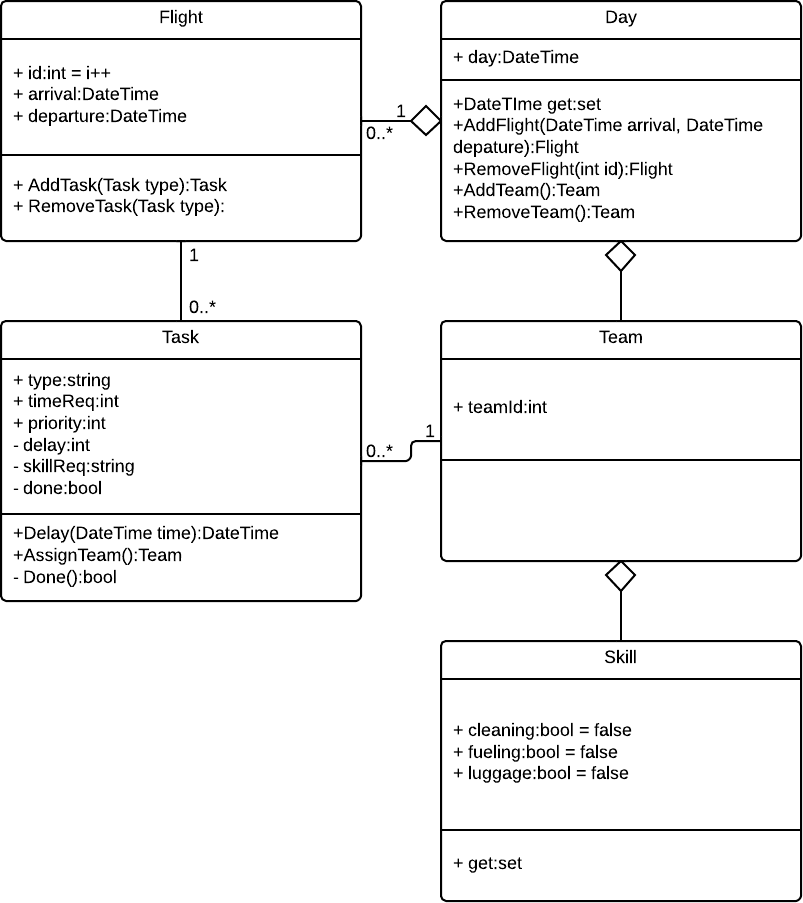
\includegraphics[width=\textwidth]{Grafik/UML}
        \caption{UML example}
        \label{UML}
        \end{figure}

    \part{Product Development}
    
    \printbibliography

\end{document}